\section{Faltungsprodukt}

Bei LTI-Systemen wird das Faltungsprodukt benötigt, um aus der Impulsantwort  $y_{\delta} = y_{\delta}(t)$ und der Anregungsfunktion 
$x = x(t)$ das Ausgangssignal $y = y(t)$ zu berechnen.


\subsection{Definition des Faltungsprodukts}

\renewcommand{\arraystretch}{2}
\begin{tabular}{ll}
    Allgemein:  & $ (f * g)(t) = \int\limits_{-\infty}^{\infty} f(\tau) \cdot g(t - \tau) \, \diff \tau$                            \\
    LTI-System: & $y(t) = (x * y_{\delta} )(t) = \int \limits_{-\infty}^{\infty} x(\tau) \cdot y_{\delta}(t - \tau) \, \diff \tau $ 
\end{tabular}
\renewcommand{\arraystretch}{1}


\subsection{Eigenschaften des Faltungsprodukts} 

\begin{itemize}
    \item Faltungsprodukt ist kommutativ \textrightarrow\ $(f * g)(t) = (g * f)(t)$
    \item Dirac-Funktion $\delta(t)$ als neutrales Element \\   
        $\delta(t - t_0) * f(t) = f(t) * \delta(t - t_0) = f(t - t_0)$
\end{itemize}


\subsection{Bestimmung des Faltungsprodukts}

\example{Grafische Bestimmung des Faltungsprodukts}

Die Funktion $g(t - \tau)$ (entspricht der an der $y$-Achse gespiegelten Funktion $g(t)$) wird über die Funktion $f(t)$ geschoben. 
Das \textbf{Produkt} der Funktionswerte \textbf{zu jedem Zeitpunkt} $t$ ergibt das Faltungsprodukt.


\begin{minipage}{0.45\columnwidth}
    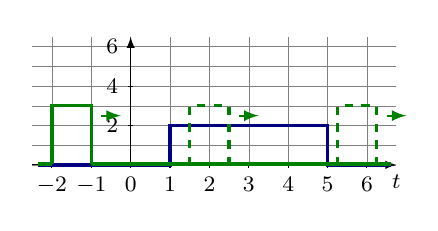
\begin{tikzpicture}
    [
    x=1cm, y=0.5cm, scale=0.5, font=\footnotesize, >=latex 
    %Voreinstellung für Pfeilspitzen
    ]
    
    %Raster im Hintergrund
    \draw[step=1, gray, very thin] (-2.5,0) grid (6.75,6.5);
    
    %Zahlen auf x-Achse
    \foreach \x in {-2,-1,0,1,2,3,4,5,6}
    \draw[shift={(\x,0)},color=black] (0pt,2pt) -- (0pt,-2pt) node[below]
    {\footnotesize $\x$};
    
    %Länge x Achse
    \draw [-latex] (-2.5,0) -- ++(9.25,0) node[below] {$t$};
    
    %Länge y Achse
    \draw [-latex] (0,0) -- ++(0,6.5) node[left] {$ $};
    
    %Zahlen auf y-Achse 
    %\foreach \y in {0,...,1}
    \foreach \y in {2,4,6}
    \draw[shift={(0,\y)},color=black] (2pt,0pt) -- (-2pt,0pt) node[left]
    {\footnotesize $\y$};		
    
    %f(t)
    \draw[blue!50!black, very thick] (-2.35,0) -- (1,0) -- (1,2) -- (5,2) -- (5,0) -- (6.6,0); 
    
    %g(t)
    \draw[green!50!black, very thick] (-2,0.05) -- (-2,3) -- (-1,3) -- (-1,0.05); 
    \draw[-latex,green!50!black, thick] (-0.75,2.5) -- (-0.25,2.5);
    
    \draw[green!50!black, very thick] (-2.35,0.05) -- (-2,0.05); 
    \draw[green!50!black, very thick] (-1,0.05) -- (6.6,0.05);		
    
    \draw[dashed, green!50!black, very thick] (1.5,0) -- (1.5,3) -- (2.5,3) -- (2.5,0); 
    \draw[-latex,green!50!black, thick] (2.75,2.5) -- (3.25,2.5);
    
    \draw[dashed, green!50!black, very thick] (5.25,0) -- (5.25,3) -- (6.25,3) -- (6.25,0); 
    \draw[-latex,green!50!black, thick] (6.5,2.5) -- (7,2.5);		
        
    
    %Vektor a
    %\draw[-latex, thick] (0,0) -- (2,3) node [midway, above] {$\vec{a}$} node (a) {}; 
    %Vektor b
    %\draw[-latex, thick] (0,0) -- (3,0) node [midway, above] {$\vec{b}$} node (b) {}; 
    %\draw[dashed] (a.center) -- ++ (3,0) node (c) {};
    %\draw[dashed] (b.center) -- ++ (2,3);
    %\draw[very thick, red, -latex] (0,0) -- (c.center) node [midway, above] {$\vec{c}$};
\end{tikzpicture}
\end{minipage}
\hfill
\begin{minipage}{0.45\columnwidth}
    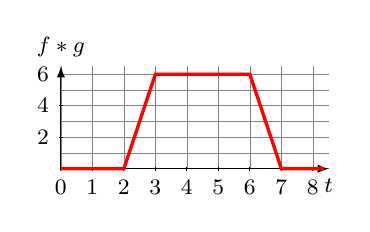
\begin{tikzpicture}
    [
    x=1cm, y=0.5cm, scale=0.4, font=\footnotesize, >=latex 
    %Voreinstellung für Pfeilspitzen
    ]
    
    %Raster im Hintergrund
    \draw[step=1, gray, very thin] (0,0) grid (8.5,6.5);
    
    %Zahlen auf x-Achse
    \foreach \x in {0,1,2,3,4,5,6,7,8}
    \draw[shift={(\x,0)},color=black] (0pt,2pt) -- (0pt,-2pt) node[below]
    {\footnotesize $\x$};
    
    %Länge x Achse
    \draw [-latex] (0,0) -- ++(8.5,0) node[below] {$t$};
    
    %Länge y Achse
    \draw [-latex] (0,0) -- ++(0,6.5) node[above] {$f*g$};
    
    %Zahlen auf y-Achse 
    %\foreach \y in {0,...,1}
    \foreach \y in {2,4,6}
    \draw[shift={(0,\y)},color=black] (2pt,0pt) -- (-2pt,0pt) node[left]
    {\footnotesize $\y$};
    
    %f(t)
    \draw[red, very thick] (0,0) -- (2,0) -- (3,6) -- (6,6) -- (7,0) -- (8.35,0); 
\end{tikzpicture}
\end{minipage}


\example{Rechnerische bestimmung des Faltungsprodukts}

\textbf{WICHTIG: Immer die einfacher definierte Funktion als $\bm{g(t - \tau)}$ wählen!} \\
(\textrightarrow\ kommutativ)

\vspace{0.2cm}

\begin{minipage}[t]{0.45\columnwidth}
    $f(t) = \begin{cases}
    2 & \text{für } \, 0 < t < 4 \\
    0 & \text{sonst}
    \end{cases}$  
\end{minipage}
\hfill
\begin{minipage}[t]{0.5\columnwidth}
    $g(t) = \begin{cases}			
    3 & \text{für } \, 0 < t < 1 \\
    0 & \text{sonst}
    \end{cases}$  	
\end{minipage}

\vspace{0.2cm}

\begin{enumerate}
    \setlength{\itemsep}{5pt} % adjust space between items

    \item \textbf{Variablentransformation}
    
    \vspace{0.2cm}

    \begin{minipage}[t]{0.45\columnwidth}
        $f(\tau) = \begin{cases}			
        2 & \text{für } \, 0 < \tau < 4 \\
        0 & \text{sonst}
        \end{cases}$ 
    \end{minipage}
    \hfill
    \begin{minipage}[t]{0.5\columnwidth}
        $g(t - \tau) = \begin{cases}			
        3 & \text{für } \, 0 < t - \tau < 1 \\
        0 & \text{sonst}
        \end{cases}$ 
    \end{minipage}

    \item  \textbf{Nach $\bm{\tau}$ auflösen (speziell bei $\bm{g(t - \tau)}$)}
        $$ 0 < t - \tau < 1 \quad \text{ \textrightarrow\ } \quad 0 - t < - \tau < 1 - t  \quad \text{ \textrightarrow\ } \quad \cgn{t} > \tau > \cgn{t - 1} $$

    \item \textbf{Hilfsdiagramm zeichnen}
    \begin{center}
        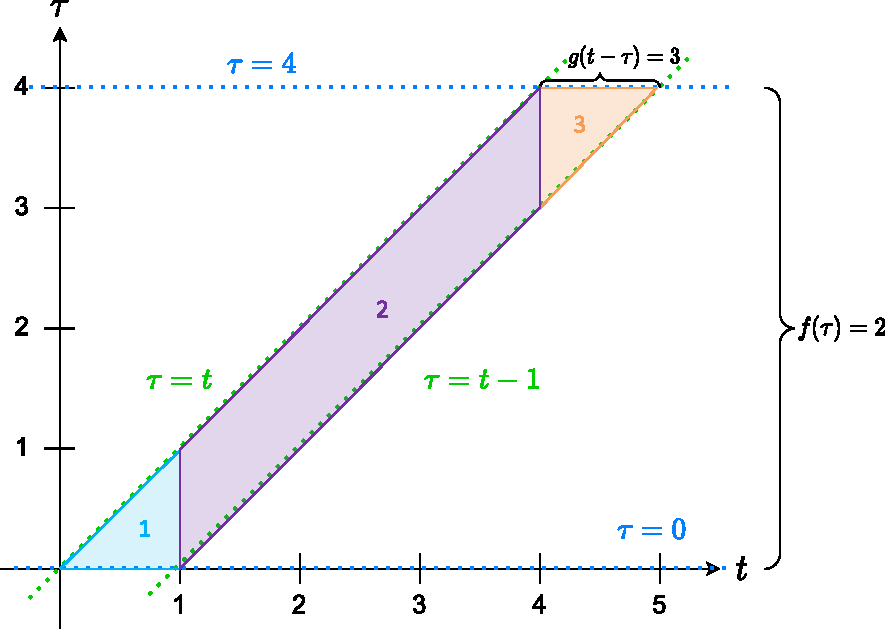
\includegraphics[width=0.85\columnwidth]{images/hilfsdiagramm.pdf}
    \end{center}
    
    \columnbreak

    \item \textbf{Faltungsprodukt abschnittweise berechnen}

    \renewcommand{\arraystretch}{2.5}
        \begin{tabular}{ll}
            $0 \leq t < 1$  & $(f * g)(t) = \int\limits_0^t 2 \cdot 3 \, \diff \tau$         \\
            $1 \leq t < 4$  & $(f * g)(t) = \int\limits_{t-1}^t 2 \cdot 3 \, \diff \tau$     \\
            $4 \leq t < 5$  & $(f * g)(t) = \int\limits_{t-1}^4 2 \cdot 3 \, \diff \tau$     \\
            sonst           & $(f * g)(t) = 0$
        \end{tabular}
    \renewcommand{\arraystretch}{1}
\end{enumerate}

